\section{Experimental results}
\label{section:results} We have implemented the algorithms with
multi-threading support from C++ 11, and conducted the experiments on
Linux PCs with Intel Core i7 4790 processor with 4 cores. We have used
the Graph-cuts optimization code written by Veksler, using the libraries
provided by Boykov and
Kolmogorov~\cite{middlebury_mrf,alpha_expansion,what_energy_can_be_min_by_gc,mrf_experimental}.
% [2] Fast Approximate Energy Minimization via Graph Cuts.
%         Y. Boykov, O. Veksler, and R. Zabih.
%         In IEEE Transactions on Pattern Analysis and Machine Intelligence
%         (PAMI), vol. 23, no. 11, pages 1222-1239, November 2001.  
%
%     [3] What Energy Functions can be Minimized via Graph Cuts?
%         V. Kolmogorov and R. Zabih. 
%         In IEEE Transactions on Pattern Analysis and Machine Intelligence
%         (PAMI), vol. 26, no. 2, pages 147-159, February 2004. 
%         An earlier version appeared in European Conference on Computer
%         Vision (ECCV), May 2002.
%
%     [4] An Experimental Comparison of Min-Cut/Max-Flow Algorithms for
%         Energy Minimization in Vision. 
%         Y. Boykov and Vladimir Kolmogorov.
%         In IEEE Transactions on Pattern Analysis and Machine Intelligence
%         (PAMI), vol. 26, no. 9, pages 1124-1137, September 2004. 
We have used the QPBO and TRW-S implementations by
Kolmogorov~\cite{QPBO, TRW-S}. We have used 4 threads
for experiments unless indicated. We now look at our experimental
results for the three problems.



% To evaluate the effectness of different parallel structures, we plot
% the energy minimization process against time. We define the energy of
% a parallel optimization system at a certain time as the minimum energy
% of all threads at that time.

\mysubsubsection{Stereo}

We performed our experiments on the Book sequence from Middlebury stereo
datasets.~\cite{middlebury_stereo}. We use 7 images with the
resolution of $695\times555$ and optimize for 256 disparity labels. We
recoreded both single thread energy and system energy (minimum energy
so far from all threads) against time. Since the order of labels to be
expanded or fused will have impact on minimization, we randomly
shuffled 256 labels and provide this order to all methods.

\begin{figure}[tb]
  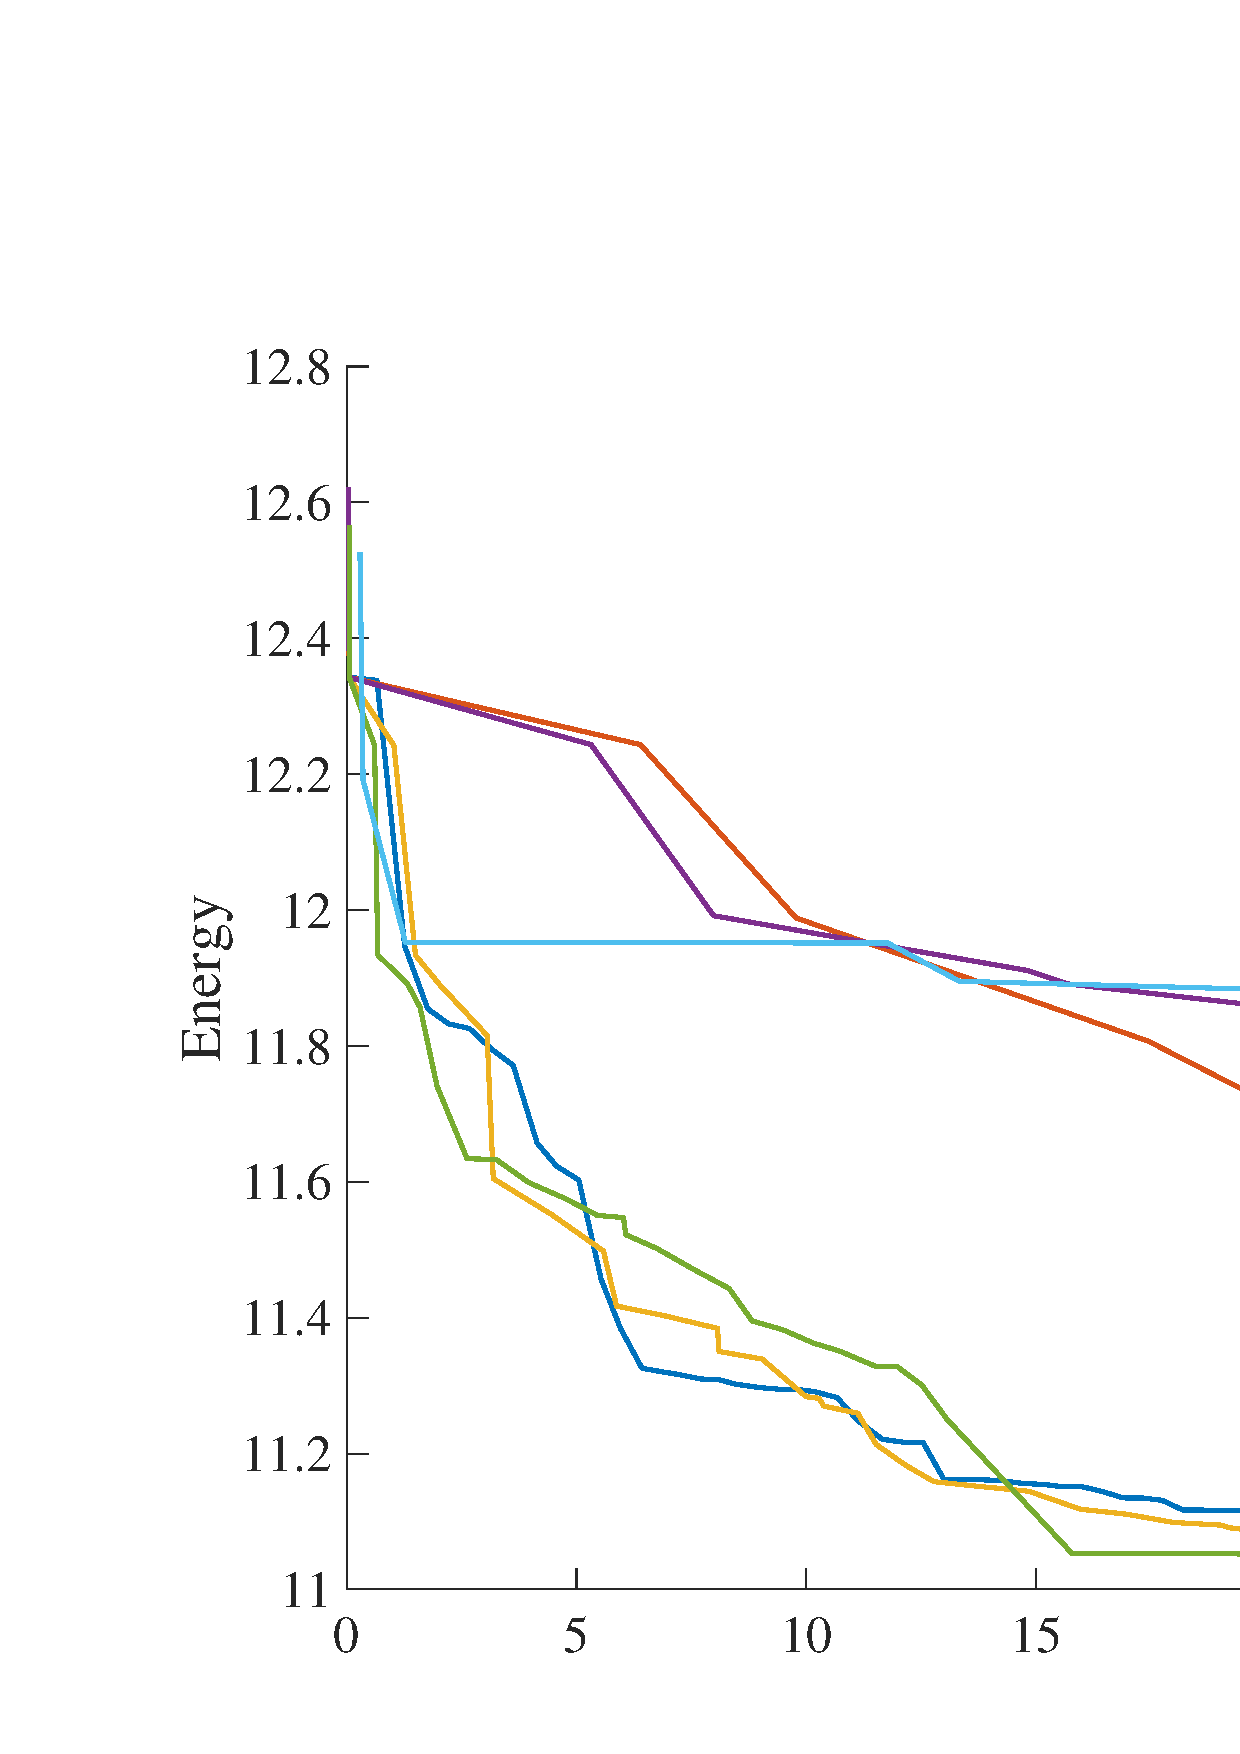
\includegraphics[width=\columnwidth]{figure/stereo_global.png}
  \caption{The energy minimization process of difference parallel systems.}
  \label{fig:stereo_global}
\end{figure}

\begin{figure}[tb]
  \includegraphics[width=\columnwidth]{figure/stereo_threads.png}
  \caption{Per thread energy. The left and right figures show the
    energy minimization process on each working thread of our method
    in SF-MF configuration and parallel $\alpha$-expansion method,
    respectively. The energy is in $\log$ scale}
  \label{fig:stereo_threads}
\end{figure}


Figure \ref{fig:stereo_global} shows the energy minimization process
against time. In this experiment, both PAE and SF-MF converge faster
than sequential method. However, since fusing solutions with multiple
labels by QPBO is slower than a single $\alpha$-expansion, PAE method
reaches convergence faster than SF-MF. Architectures with multiway
fusion, e.g. SF and SF-SS perform worse than PAE and SF-MF, because
the TRWS algorihtm used in multiway fusion is slower than multiple
$\alpha$-expansion. Finally, the line of hierarchy fusion only makes
jump when fusing on root node of the tree. This is because any fusion
step on non-root nodes only have partial label information.

Figure \ref{fig:stereo_threads} shows the per-thread energy
minimization process in SF-MF and PAE. The per-thread energy in SF-MF
architecture decreases more uniformly than that of PAE. In the
scenario where we need to query the best solution so far before the
whole optimization converges, SF-MF architecture is a better choice.

For a easy optimization problem as shown in this section, our full
architecture with solution sharing and multiway fusion actually makes
convergence slower by adopting sophisticated algorihtm and introducing
multi-threading overhead. However, we can easily configure the
architecture to make it better fit the problem, e.g. turn off multiway
fusion and/or solution sharing.


\mysubsubsection{Optical Flow}

\noindent
%
We have chosen the Dimetrodon image pair from the Middlebury flow
dataset~\cite{middlebury_optical_flow}. Figure~\ref{fig:optical_flow_convergence}
shows the energy plots of the three competing methods, Fusion Move
(FM), Parallel Fusion Move (PFM), and Hierarchical Fusion Move (HFM),
against our Swarm Fusion methods (SF-MF, SF-SS, SF). A key observation
is that SF-MF converges quicker and better than PFM. This is indeed the
benefits of solution sharing in our network. Optical flow is a more
difficult problem and many solution proposals are not effective.
The solution sharing (i.e., SF-MF) allows all the threads to exchange
effective solution proposals in the middle of the
optimization.

\begin{figure}[!h]
  \centering
  \includegraphics[width=0.8\columnwidth]{figure/optical_flow_convergence.png}
  \caption{Energy plots for optical flow estimation. SF-MF has the best
 performance due to its solution sharing strategy.}\label{fig:optical_flow_convergence}
\end{figure}

\begin{figure}[!h]
  \centering
  \begin{subfigure}[b]{0.49\columnwidth}
    \centering
    \includegraphics[width=\columnwidth]{figure/optical_flow_PFM_threads.png}
    \caption{}
    \label{fig:optical_flow_PFM_threads}
  \end{subfigure}  
  \begin{subfigure}[b]{0.49\columnwidth}
    \centering
    \includegraphics[width=\columnwidth]{figure/optical_flow_SF_MF_threads.png}
    \caption{}
    \label{fig:optical_flow_SF_MF_threads}
  \end{subfigure}
  \caption{Energy plots per thread for (a) Parallel Fusion  
    Move (PFM) and (b) our FS-MF.}
  \label{fig:optical_flow_by_threads}  
\end{figure}

% 
% This is because some solution proposals are more effective than others,
% so once a thread grabs an effective solution proposal, it find a lower
% energy quickly. Since there is no solution sharing in PFM model, other
% threads cannot share this lower energy state, and keeps working on its
% own state.
%
%On the other hand, SF-MF
%allows solution sharing, so once a thread grabs an effective solution
%proposal and moves to a lower energy state, other threads can share
%information about this lower energy state. In this manner, all threads
%contribute to further decrease of this low energy state. To further
%demonstrate what is happening here,
To further investigate the effectiveness of solution sharing,
Figure~\ref{fig:optical_flow_by_threads} shows the energy plots of PFM
and SF-MF per thread. As evident from the plot, in PFM, one thread found
a better solution than others, but other threads keep working
independently at higher energy states. SF-MF, on the other hand,
exchanges solutions all the time, and every thread is making an effective
work in improving the solution.
%As we can see from the plots, in PFM model, one thread finds lower
%energy state faster than others, while other threads keep working at
%their own energy state. But in SF-MF model, all threads exchange
%information about the lowest energy state frequently and work on
%improving the lowest energy state together. Since the solution for
%optical flow can be locally improved by each thread, the final merging
%of PFM can effectively fuse good local results in different threads
%together and achieve a similar energy state with SF-MF model. But as
%SF-MF model shares information in the middle, a final merging becomes
%less necessary.
Another key finding from Fig.~\ref{fig:optical_flow_convergence} is that
SF is slower than SF-MF. Our analysis is that multi-way fusion is
inefficient in this problem setting, since solution proposals are
relatively independent and fusing the solution space would not gain much
benefit. It rather loses performance against QPBO~\cite{QPBO} due to the
overhead of TRW-S.

There are two factors influencing solution sharing: 1) \textit{the
number of solutions to share} and 2) \textit{the frequency of solution
sharing}. Both factors are controlled by $\beta$. As mentioned in
Section~\ref{section:algorithm}, we have used $\beta = 1$ (i.e., share
solutions) once in every five iterations.  To further understand the
effects of solution sharing, we did two more experiments. First, we set
$\beta$ to 0, 1, 2, or 3 in every five iterations,
% (when $\beta = 0$, it is the same with PFM without final merging).
while keeping all other parameters the same (See
Fig.~\ref{fig:optical_flow_by_beta}).  Second, we change the number of
iterations $k$ between the two consecutive solution sharing iterations
(See Fig.~\ref{fig:optical_flow_by_interval}).  The first experiment
revealed that the solution sharing makes convergence faster regarless of
$\beta$.  However, too much solution sharing slows down the converence,
and $\beta=1$ is the sweet spot for this problem.
%
% , energy generally
% decreases faster with solution sharing. But since we need to perform one
% fusion for sharing each solution, sharing more solution decreases
% efficiency in this problem setting. While sharing multiple solutions
% might be useful in some other problem setting as it means each thread
% can get more global information early.
%
The second experiment has shown that too frequent solution sharing
harms the convergence, simply because we have less time generating more
proposals and exploring the solution space.
% From this figure, we can see that
% although solution sharing generally speeds up the optimization process,
% sharing solution too frequently is not a good practice. This is because
% when we share solution frequently, we have less time for generating and
%fusing new proposals.
Optimal parameter setting depends on each problem setting.
%A good choice of the solution sharing frequency depends on specific
%problem setting.


\begin{figure}[!h]
  \centering
  \begin{subfigure}[b]{0.49\columnwidth}
    \centering
    \includegraphics[width=\columnwidth]{figure/optical_flow_by_beta.png}
    \caption{}
    \label{fig:optical_flow_by_beta}
  \end{subfigure}  
  \begin{subfigure}[b]{0.49\columnwidth}
    \centering
    \includegraphics[width=\columnwidth]{figure/optical_flow_by_interval.png}
    \caption{}
    \label{fig:optical_flow_by_interval}
  \end{subfigure}
  \caption{Energy plots for optical flow with (a) varying
    $\beta$ and (b) varying solution sharing
    frequencies. Solution sharing achieves better convergence, but sharing too many solutions (larger $\beta$) or sharing solutions too frequently (less $k$) slows down the convergence, as it reduces the time for exploration.}
\end{figure}

\mysubsubsection{Layered depthmap estimation}

\noindent We have used ``ours\_1'' data in~\cite{layered_depthmap} for
the experiments. Figure~\ref{fig:layered_depthmap_convergence} shows
that Fusion Move, Parallel Fusion Move and SF-MF all got stuck in local
minima, which is due to the lack of multi-way fusion.  Layered depthmap
estimation is a challenging problem with very large solution space. The
binary fusion of solution proposals is too restrictive to make any
improvements.  This coincides with the observation in
\cite{layered_depthmap} that binary fusion of proposal solutions is not
as powerful as their subspace fusion which is a special form of
multi-way fusion here. Lastly, solution sharing also plays an important
role for this challenging problem for exactly the same reason, as SF
performs much better than SF-SS.
%
%From the plot, we can see that, Fusion Move, Parallel Fusion Move, and
%SF-MF all stalk at a high energy state.
To further study the effects of multi-way fusion, we have varied the
value of $\alpha$ in controlling the number of solution proposals to be
fused in SF-SS model (See
Fig.~\ref{fig:layered_depthmap_by_alpha}). Note that we have used SF-SS
instead of SS to disable solution sharing and better observe the effects
of multi-way fusion.
% SF-SS model (disable solution sharing to
%better observe the effect of multi-way fusion) while keeping other
%parameters the same and plot the energy minimization process in figure
It is interesting to see that more multi-way fusion takes longer to
converge, but finds a lower energy state at the end.
%We can see that as the number of
%ways to fuse becomes larger, each fusion step takes longer time, but the
%chance of finding a lower energy state increases.

\begin{figure}[tb]
  \includegraphics[width=\columnwidth]{figure/layered_depthmap_convergence.png}
  \caption{Energy plots for the layered depthmap estimation
 problem. Both the multi-way fusion and the solution sharing are important
 for this challenging problem.}\label{fig:layered_depthmap_convergence}
\end{figure}
\begin{figure}[tb]
  \includegraphics[width=\columnwidth]{figure/layered_depthmap_by_alpha.png}
 \caption{Energy plots for different values of $\alpha$.
 More multi-way fusion takes longer to converge but finds a better
 solution at the end.}\label{fig:layered_depthmap_by_alpha}
\end{figure}




%As shown in the above problem settings, the solution sharing and
%multi-way fusion enabled by our uniform framework play a key role for
%improving performance in different problem settings.

